\documentclass[12pt]{article}
\usepackage{geometry}
\usepackage{tikz}
\geometry{margin=1in}
\title{Pattern Matching Worksheet}
\author{}
\date{}

\begin{document}

\maketitle

\section*{Instructions}
Look at each pattern carefully. Choose the shape, number, or item that comes next in the pattern. Circle your answer.

\section*{Problem 1: Shape Sequence}
\begin{center}
\begin{tikzpicture}
  \node at (0,0) {\Large $\triangle$};
  \node at (1.5,0) {\Large $\square$};
  \node at (3,0) {\Large $\circ$};
  \node at (4.5,0) {\Large $\triangle$};
  \node at (6,0) {\Large $\square$};
  \node at (7.5,0) {?};
\end{tikzpicture}
\end{center}
What shape comes next?

\vspace{1em}
\noindent A) $\triangle$ \quad B) $\square$ \quad C) $\circ$ \quad D) $\star$

\section*{Problem 2: Number Pattern}
2, 4, 8, 16, \rule{1cm}{0.15mm}, \rule{1cm}{0.15mm}

\vspace{1em}
\noindent What are the next two numbers?

\vspace{1em}
\noindent A) 20, 24 \quad B) 24, 32 \quad C) 32, 64 \quad D) 32, 48

\section*{Problem 3: Picture Pattern}
\begin{center}
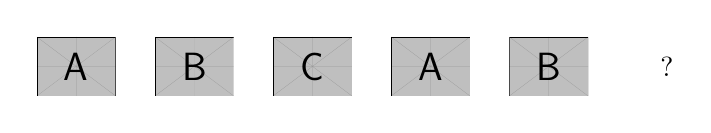
\begin{tikzpicture}
  \node at (0,0) {\includegraphics[width=1cm]{example-image-a}};
  \node at (1.5,0) {\includegraphics[width=1cm]{example-image-b}};
  \node at (3,0) {\includegraphics[width=1cm]{example-image-c}};
  \node at (4.5,0) {\includegraphics[width=1cm]{example-image-a}};
  \node at (6,0) {\includegraphics[width=1cm]{example-image-b}};
  \node at (7.5,0) {?};
\end{tikzpicture}
\end{center}
Which image comes next?

\vspace{1em}
\noindent A) \includegraphics[width=0.7cm]{example-image-c} \quad B) \includegraphics[width=0.7cm]{example-image-b} \quad C) \includegraphics[width=0.7cm]{example-image-a} \quad D) \includegraphics[width=0.7cm]{example-image}

\end{document}
